\documentclass[10pt]{beamer}\usepackage[]{graphicx}\usepackage[]{color}
%% maxwidth is the original width if it is less than linewidth
%% otherwise use linewidth (to make sure the graphics do not exceed the margin)
\makeatletter
\def\maxwidth{ %
  \ifdim\Gin@nat@width>\linewidth
    \linewidth
  \else
    \Gin@nat@width
  \fi
}
\makeatother

\definecolor{fgcolor}{rgb}{0.345, 0.345, 0.345}
\newcommand{\hlnum}[1]{\textcolor[rgb]{0.686,0.059,0.569}{#1}}%
\newcommand{\hlstr}[1]{\textcolor[rgb]{0.192,0.494,0.8}{#1}}%
\newcommand{\hlcom}[1]{\textcolor[rgb]{0.678,0.584,0.686}{\textit{#1}}}%
\newcommand{\hlopt}[1]{\textcolor[rgb]{0,0,0}{#1}}%
\newcommand{\hlstd}[1]{\textcolor[rgb]{0.345,0.345,0.345}{#1}}%
\newcommand{\hlkwa}[1]{\textcolor[rgb]{0.161,0.373,0.58}{\textbf{#1}}}%
\newcommand{\hlkwb}[1]{\textcolor[rgb]{0.69,0.353,0.396}{#1}}%
\newcommand{\hlkwc}[1]{\textcolor[rgb]{0.333,0.667,0.333}{#1}}%
\newcommand{\hlkwd}[1]{\textcolor[rgb]{0.737,0.353,0.396}{\textbf{#1}}}%
\let\hlipl\hlkwb

\usepackage{framed}
\makeatletter
\newenvironment{kframe}{%
 \def\at@end@of@kframe{}%
 \ifinner\ifhmode%
  \def\at@end@of@kframe{\end{minipage}}%
  \begin{minipage}{\columnwidth}%
 \fi\fi%
 \def\FrameCommand##1{\hskip\@totalleftmargin \hskip-\fboxsep
 \colorbox{shadecolor}{##1}\hskip-\fboxsep
     % There is no \\@totalrightmargin, so:
     \hskip-\linewidth \hskip-\@totalleftmargin \hskip\columnwidth}%
 \MakeFramed {\advance\hsize-\width
   \@totalleftmargin\z@ \linewidth\hsize
   \@setminipage}}%
 {\par\unskip\endMakeFramed%
 \at@end@of@kframe}
\makeatother

\definecolor{shadecolor}{rgb}{.97, .97, .97}
\definecolor{messagecolor}{rgb}{0, 0, 0}
\definecolor{warningcolor}{rgb}{1, 0, 1}
\definecolor{errorcolor}{rgb}{1, 0, 0}
\newenvironment{knitrout}{}{} % an empty environment to be redefined in TeX

\usepackage{alltt}
\usetheme{metropolis}           % Use metropolis theme

\usepackage{graphicx}

\DeclareGraphicsExtensions{.pdf,.jpeg,.jpg,.png}

\usepackage{subcaption}
\usepackage{amsmath}

\usepackage{tikz}
\usetikzlibrary{bayesnet}
\usepackage{pgfplots}
\pgfplotsset{compat=1.13}

\usepackage[framemethod=TikZ, xcolor=RGB]{mdframed}
\definecolor{mydarkblue}{rgb}{0,.06,.5}
\definecolor{mydarkred}{rgb}{.5,0,.1}
\definecolor{myroyalblue}{rgb}{0,.1,.8}
\mdfdefinestyle{MyFrame}{%
    linecolor=mydarkblue,
    outerlinewidth=0.5pt,
    roundcorner=2pt,
    innertopmargin=2pt,
    innerbottommargin=2pt,
    innerrightmargin=2pt,
    innerleftmargin=2pt,
    backgroundcolor=blue!10}

% Set a transparent background to match ggplot figures
\setbeamercolor{background canvas}{bg=}


% Operators
\def\mbe{\mathbb{E}}%
\def\ind#1{\mathbb{I}\left(#1\right)}
\def\evalat#1#2{\left.#1\right|_{#2}}
\def\fracat#1#2#3{\left.\frac{#1}{#2}\right\vert_{#3}}
\def\iid{\overset{iid}{\sim}}
\def\expect#1#2{\underset{#1}{\mathbb{E}}\left[#2\right]}
\def\cov#1#2{\underset{#1}{\mathrm{Cov}}\left(#2\right)}
\def\expecthat#1#2{\underset{#1}{\widehat{\mathbb{E}}}\left[#2\right]}
\def\abs#1{\left|#1\right|}
\def\norm#1{\left\Vert#1\right\Vert}
\def\norminf#1{\left\Vert#1\right\Vert_{\infty}}
\def\sumk{\sum_{\k=1}^{\kmax}}
\def\sumkm{\sum_{\k=1}^{\kmax - 1}}
\def\dirderiv#1#2{\delta_{#1\rightarrow#2}} % A directional derivative (unused?)
\def\linop{\mathcal{L}} % A linear operator

\DeclareMathOperator*{\argmax}{\mathrm{argmax}}
\DeclareMathOperator*{\argmin}{\mathrm{argmin}}
\DeclareMathOperator*{\esssup}{\mathrm{esssup}}

% Variables
\def\etaopt{\hat\eta} % Optimal vb parameters
\def\x{x}   % Data
\def\t{t}   % Generic priur parameter
\def\z{z}   % Cluster indicators
\def\g{g}   % Function of interest
\def\k{k}   % Cluster index
\def\n{n}   % Data index
\def\nuk{\nu_{\k}}   % K-th stick.  Have to type this a lot.
\def\const{C}   % Constant
\def\lnu{\tilde{\nu}}   % Unconstrained stick
\def\lnumean{\eta^{\mu}}   % Unconstrained stick vb mean
\def\lnusd{\eta^{\sigma}}   % Unconstrained stick vb std
\def\hess#1{H_{#1}}   % Hessian
\def\phiz{0_\phi}   % The phi zero function.
\def\infl{\psi}   % The influence function
\def\inflg{\psi_{\g}}   % The influence function for a function of interest

\def\etatheta{\eta_{\theta}}  % VB parameters for certain components
\def\etanu{\eta_{\nu}}  % VB parameters for certain components
\def\etanuk{\eta_{\nuk}}  % VB parameters for certain components
\def\etaz{\eta_{\z}}  % VB parameters for certain components
\def\etaglob{\eta_{\gamma}}  % VB parameters for theta and nu
\def\etaopttheta{\etaopt_{\theta}}  % VB parameters for certain components
\def\etaoptnu{\etaopt_{\nu}}  % VB parameters for certain components
\def\etaoptnuk{\etaopt_{\nuk}}  % VB parameters for certain components
\def\etaoptz{\etaopt_{\z}}  % VB parameters for certain components
\def\etaoptgamma{\etaopt_{\gamma}}  % VB parameters for certain components


% Distributions
\def\pstick{p_{\mathrm{stick}}}   % Stick breaking distribution
\def\q{q}   % VB dist
\def\logp{\ell}   % Log probabiltty
\def\lqgrad#1{{\nabla \log \q}\left(#1\right)}   % Log VB distribution gradient
\def\lqhess#1{{\nabla^2 \log \q}\left(#1\right)}   % Log VB distribution Hessian
\def\lqgradbar#1{\overline{\lqgrad{#1}}\,\,}   % Log VB distribution gradient centered
\def\lqhessbar#1{\overline{\lqhess{#1}}\,\,}   % Log VB distribution Hessian centered
\def\normdist#1{\mathcal{N}\left(#1\right)}   % Normal distribution
\def\KL#1{\mathrm{KL}\left(#1\right)}   % KL divergence
\def\KLgrad#1{\mathrm{KL}_{\eta}\left(#1\right)}   % KL divergence
\def\KLhess#1{\mathrm{KL}_{\eta\eta}\left(#1\right)}   % KL divergence
\def\wishart#1{\mathrm{Wishart}\left(#1\right)}   % Wishart distribution
\def\gammadist#1{\mathrm{Gamma}\left(#1\right)}   % Gamma distribution
\def\betadist#1{\mathrm{Beta}\left(#1\right)}   % Gamma distribution
\def\pb{p_{0}}   % Base prior
\def\pa{p_{1}}   % Alternative prior

% Taylor series
\def\etalin{\etaopt^{\mathrm{lin}}}
\def\glin{\g^{\mathrm{lin}}}
\def\gapprox{\g^{\etalin}}

% Dimensions
\def\N{N}   % Number of datapoints
\def\K{K}   % Number of components
\def\kmax{{\K_{\mathrm{max}}}}   % Truncation
\def\etadim{{D_{\eta}}}
\def\thetadim{{D_{\theta}}}
\def\zetadim{{D_{\zeta}}}
\def\ngh{N_{\mathrm{GH}}}   % Number of GH points

% Domains
\def\etadom{\Omega_{\eta}}
\def\thetadom{\Omega_{\theta}}
\def\tdom{\Omega_{\t}}
\def\linf{{L_{\infty}[0,1]}}
\def\ball{\mathcal{B}}

% Annotations
\def\mathtxt#1{\quad\textrm{#1}\quad}%
\def\mathand{\quad\textrm{and}\quad}%
\def\mathwhere{\quad\textrm{where}\quad}%
\def\constdesc#1{\textrm{(}\const\textrm{ does not depend on }#1\textrm{)}}
\def\assuitemref#1#2{\assuref{#1} (\itemref{#2})}%



\title{Evaluating Sensitivity to the Stick Breaking Prior in
Bayesian Nonparametrics}
\author{}
\date{April 26, 2021}
\institute{University of California, Berkeley}

\setbeamertemplate{Collaborators}[none]
\IfFileExists{upquote.sty}{\usepackage{upquote}}{}
\begin{document}
\maketitle


%%%%%%%%%%%%%%%%%%%%%%%%%%%%%%%%%%%%%%
%%%%%%%%%%%%%%%%%%%%%%%%%%%%%%%%%%%%%%
% Do not edit the TeX file your work
% will be overwritten.  Edit the RnW
% file instead.
%%%%%%%%%%%%%%%%%%%%%%%%%%%%%%%%%%%%%%
%%%%%%%%%%%%%%%%%%%%%%%%%%%%%%%%%%%%%%




\newcommand{\FunctionPathsMultFig}{

%<<mult_path, cache=cache, fig.show='hold', fig.cap=fig_cap>>=
\begin{knitrout}
\definecolor{shadecolor}{rgb}{0.969, 0.969, 0.969}\color{fgcolor}

{\centering 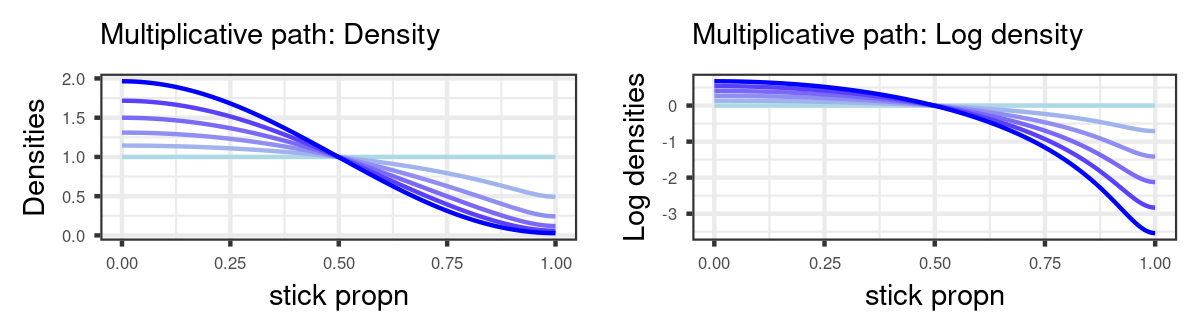
\includegraphics[width=0.980\linewidth,height=0.274\linewidth]{figure/mult_path-1} 

}



\end{knitrout}
}


\newcommand{\FunctionPathsLinFig}{

%<<lin_path, cache=cache, fig.show='hold', fig.cap=fig_cap>>=
\begin{knitrout}
\definecolor{shadecolor}{rgb}{0.969, 0.969, 0.969}\color{fgcolor}

{\centering 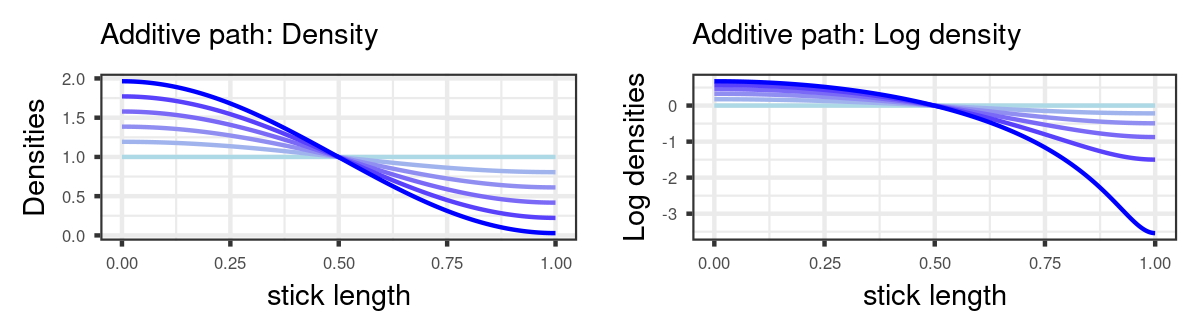
\includegraphics[width=0.980\linewidth,height=0.274\linewidth]{figure/lin_path-1} 

}



\end{knitrout}
}


\newcommand{\FunctionBallFig}{

\begin{knitrout}
\definecolor{shadecolor}{rgb}{0.969, 0.969, 0.969}\color{fgcolor}\begin{figure}[!h]

{\centering 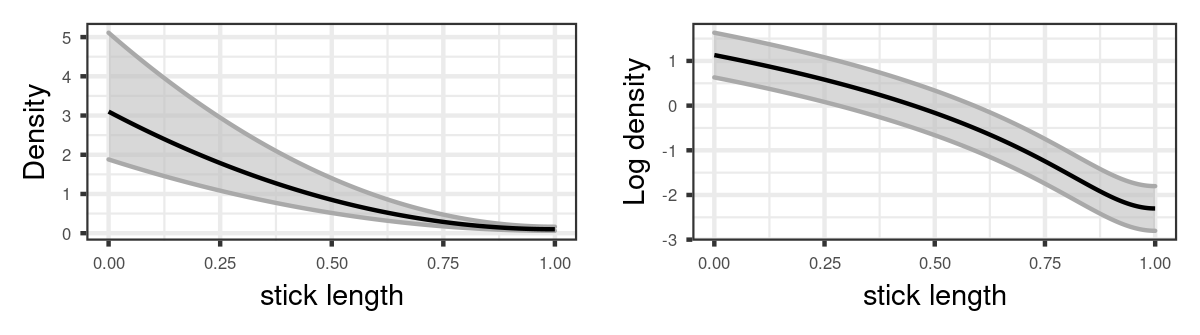
\includegraphics[width=0.980\linewidth,height=0.274\linewidth]{figure/func_ball-1} 

}

\caption[An $\linf{\cdot}$ ball]{An $\linf{\cdot}$ ball.}\label{fig:func_ball}
\end{figure}


\end{knitrout}
}




\newcommand{\FunctionDistFig}{

\begin{knitrout}
\definecolor{shadecolor}{rgb}{0.969, 0.969, 0.969}\color{fgcolor}

{\centering 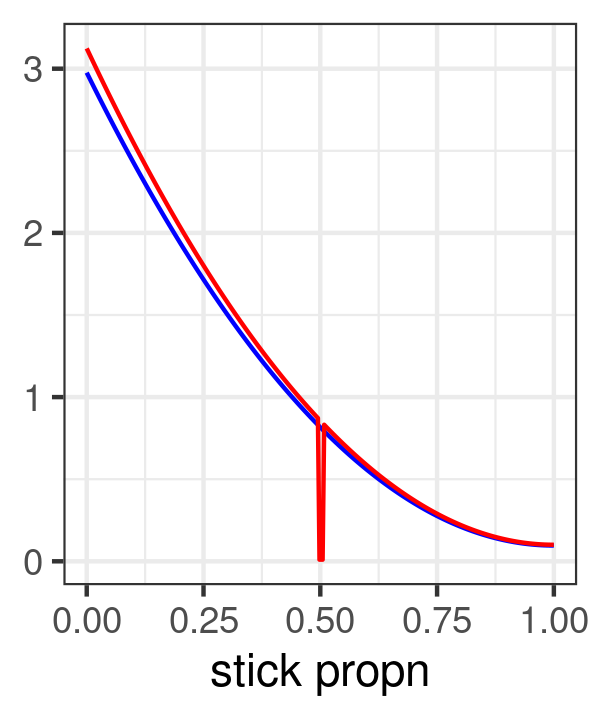
\includegraphics[width=0.490\linewidth,height=0.588\linewidth]{figure/func_dist-1} 

}



\end{knitrout}
}

%%%%%%%%%%%%%%%%%%%%%%%%%%%%%%%%%%%%%%
%%%%%%%%%%%%%%%%%%%%%%%%%%%%%%%%%%%%%%
% Do not edit the TeX file your work
% will be overwritten.  Edit the RnW
% file instead.
%%%%%%%%%%%%%%%%%%%%%%%%%%%%%%%%%%%%%%
%%%%%%%%%%%%%%%%%%%%%%%%%%%%%%%%%%%%%%




%%%%%%%%%%%%%%%%%%%%%%%%%%%%%
% initial fit for iris
%%%%%%%%%%%%%%%%%%%%%%%%%%%%%
\newcommand{\IrisFit}{

\begin{knitrout}
\definecolor{shadecolor}{rgb}{0.969, 0.969, 0.969}\color{fgcolor}

{\centering 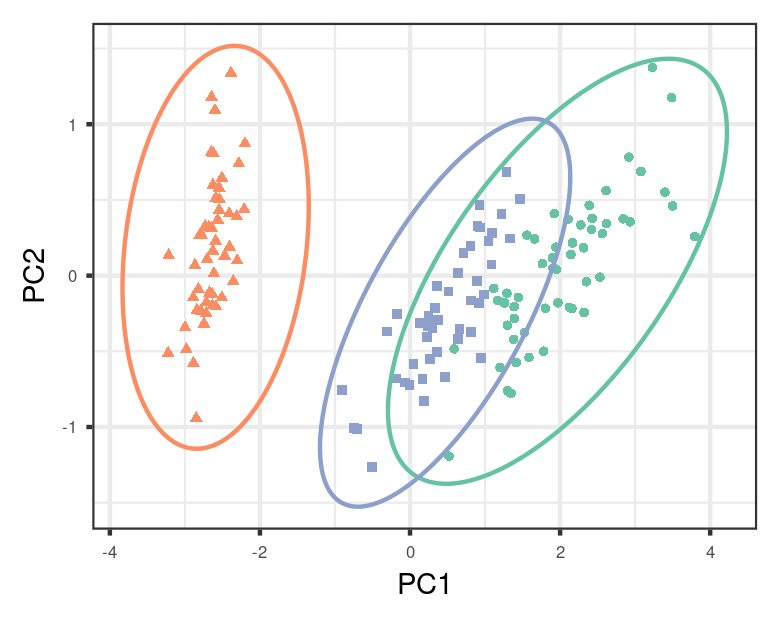
\includegraphics[width=0.637\linewidth,height=0.510\linewidth]{figure/iris_init-1} 

}



\end{knitrout}
}

%%%%%%%%%%%%%%%%%%%%%%%%%%%%%
% iris alpha sensitivity
%%%%%%%%%%%%%%%%%%%%%%%%%%%%%
\newcommand{\IrisAlphaRefit}{


\begin{knitrout}
\definecolor{shadecolor}{rgb}{0.969, 0.969, 0.969}\color{fgcolor}

{\centering 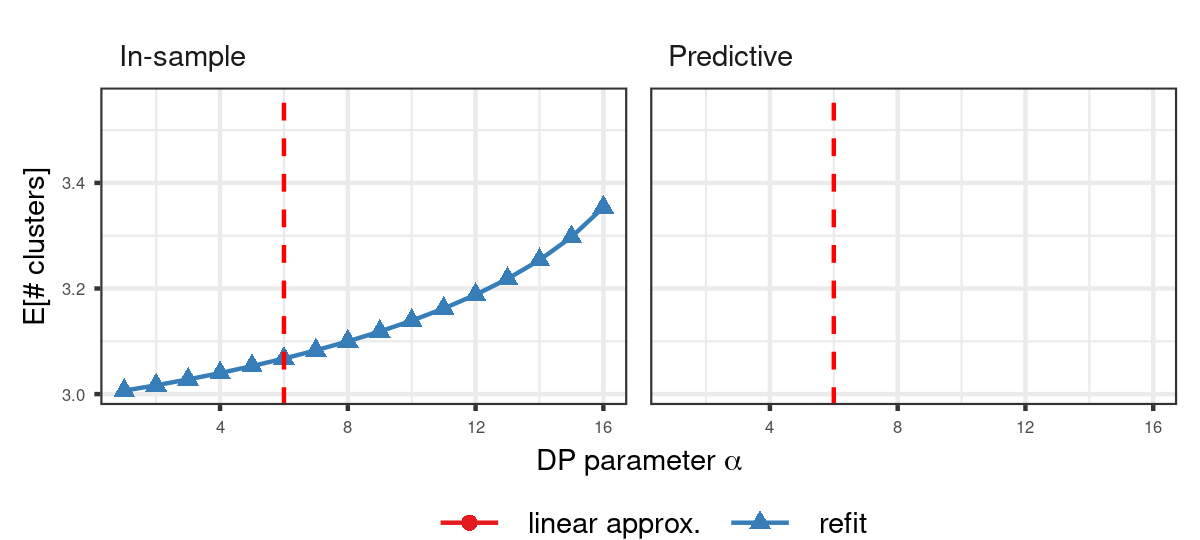
\includegraphics[width=0.980\linewidth,height=0.441\linewidth]{figure/iris_alphasens_refit-1} 

}



\end{knitrout}
}

\newcommand{\IrisAlphaInSample}{
\begin{knitrout}
\definecolor{shadecolor}{rgb}{0.969, 0.969, 0.969}\color{fgcolor}

{\centering 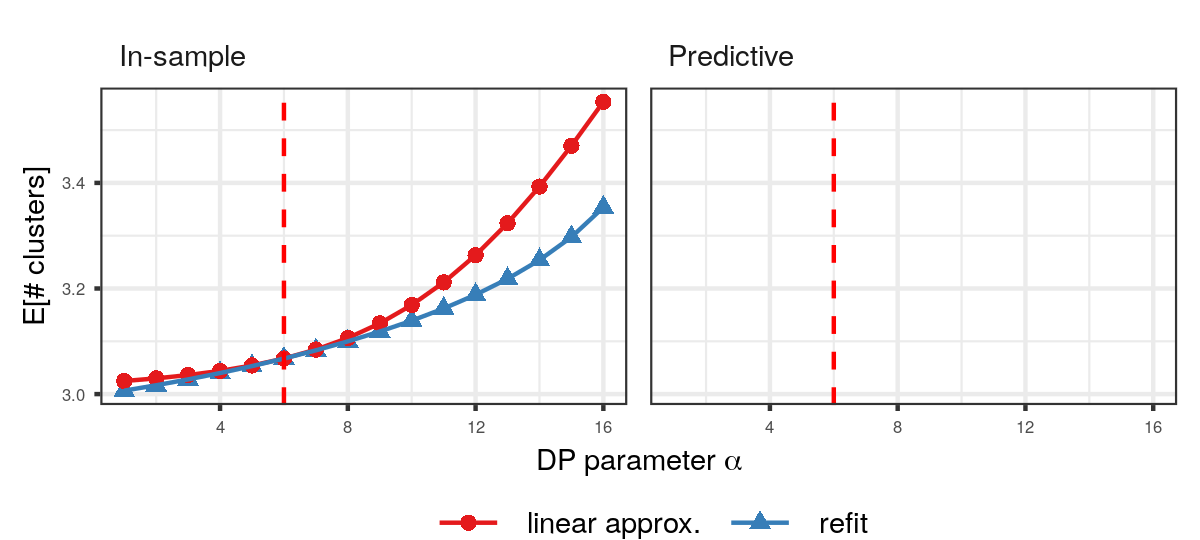
\includegraphics[width=0.980\linewidth,height=0.441\linewidth]{figure/iris_alphasens_insample-1} 

}



\end{knitrout}
}

\newcommand{\IrisAlphaAll}{
\begin{knitrout}
\definecolor{shadecolor}{rgb}{0.969, 0.969, 0.969}\color{fgcolor}

{\centering 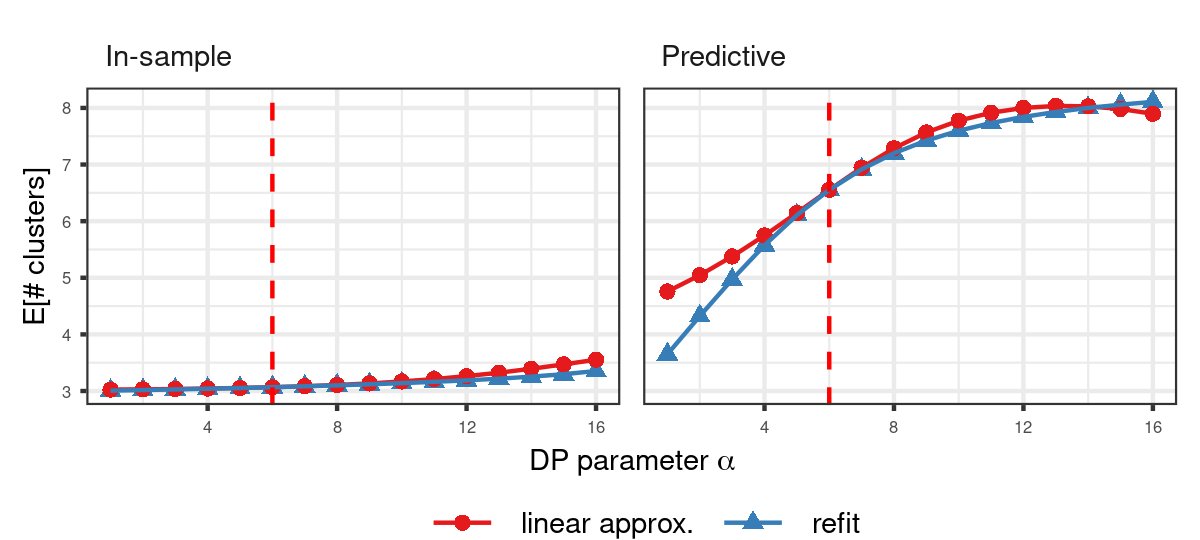
\includegraphics[width=0.980\linewidth,height=0.441\linewidth]{figure/iris_alphasens_all-1} 

}



\end{knitrout}
}


%%%%%%%%%%%%%%%%%%%%%%%%%%%%%
% iris influence function
%%%%%%%%%%%%%%%%%%%%%%%%%%%%%
\newcommand{\IrisInfluence}{

\begin{knitrout}
\definecolor{shadecolor}{rgb}{0.969, 0.969, 0.969}\color{fgcolor}

{\centering 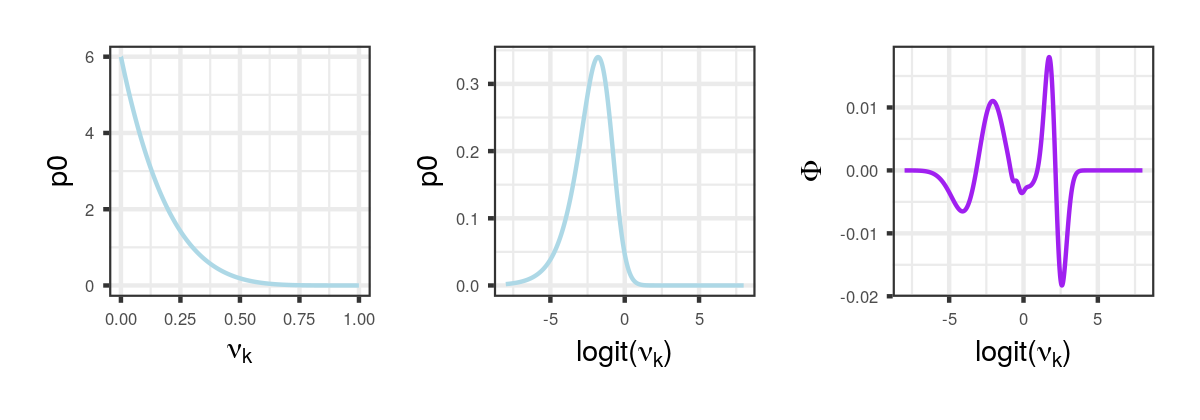
\includegraphics[width=0.980\linewidth,height=0.343\linewidth]{figure/iris_infl-1} 

}



\end{knitrout}
}


%%%%%%%%%%%%%%%%%%%%%%%%%%%%%
% iris function perturbations
%%%%%%%%%%%%%%%%%%%%%%%%%%%%%
\newcommand{\IrisFpertEx}{

\begin{knitrout}
\definecolor{shadecolor}{rgb}{0.969, 0.969, 0.969}\color{fgcolor}

{\centering 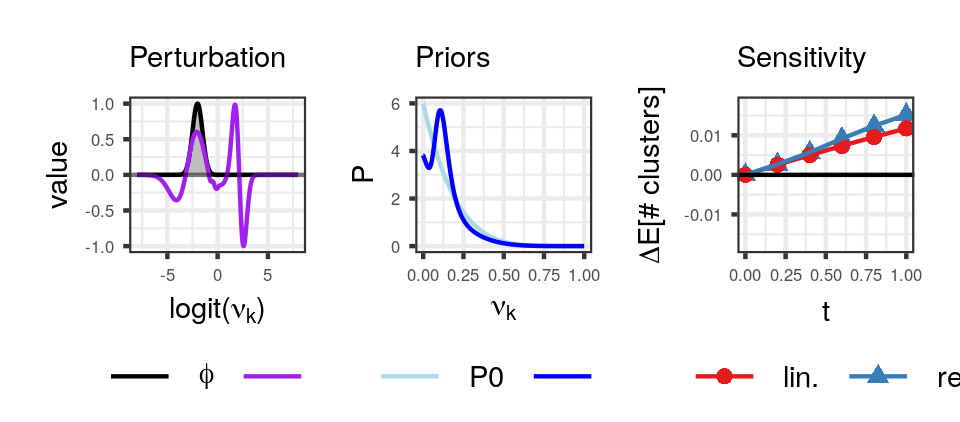
\includegraphics[width=0.784\linewidth,height=0.345\linewidth]{figure/iris_fpertex-1} 

}



\end{knitrout}
}

\newcommand{\IrisFpertAll}{

\begin{knitrout}
\definecolor{shadecolor}{rgb}{0.969, 0.969, 0.969}\color{fgcolor}

{\centering 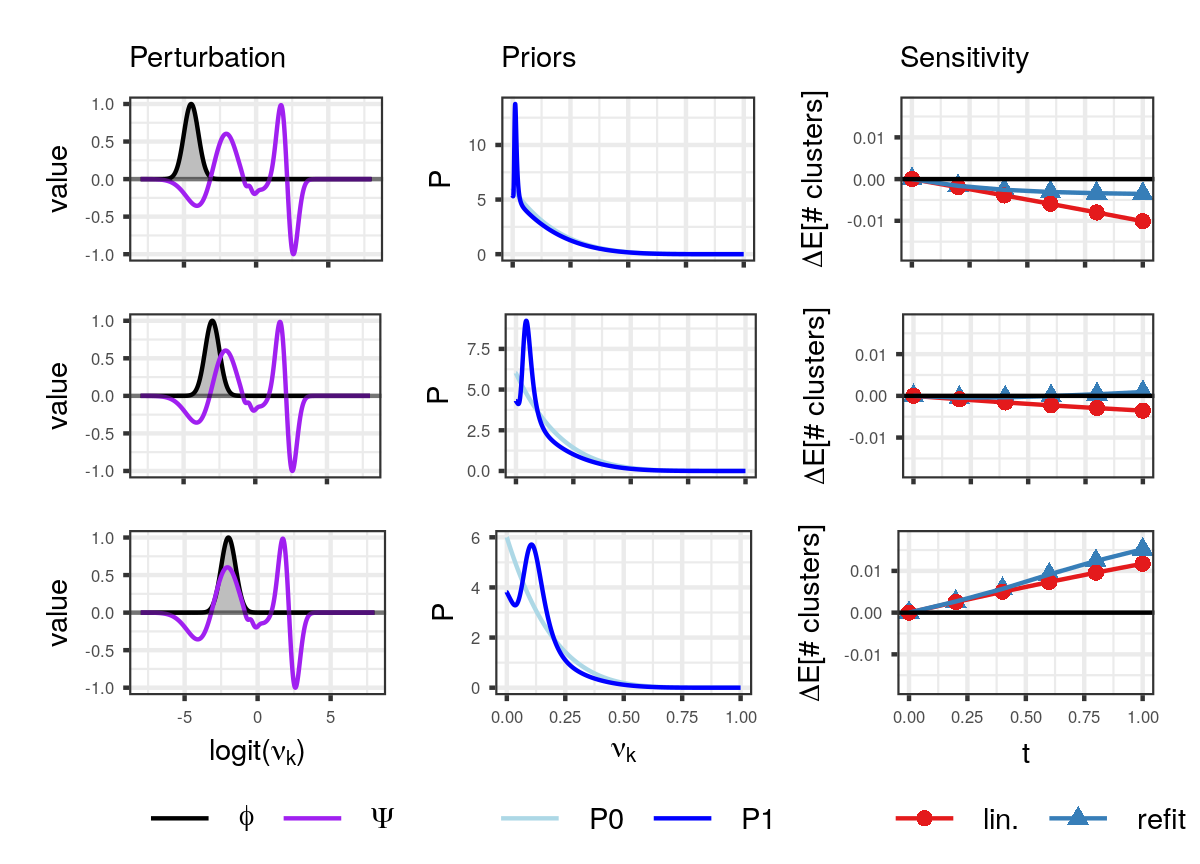
\includegraphics[width=0.784\linewidth,height=0.690\linewidth]{figure/iris_fpertall-1} 

}



\end{knitrout}
}


%%%%%%%%%%%%%%%%%%%%%%%
% iris worst-case
%%%%%%%%%%%%%%%%%%%%%%%%
\newcommand{\IrisWorstCase}{

\begin{knitrout}
\definecolor{shadecolor}{rgb}{0.969, 0.969, 0.969}\color{fgcolor}

{\centering 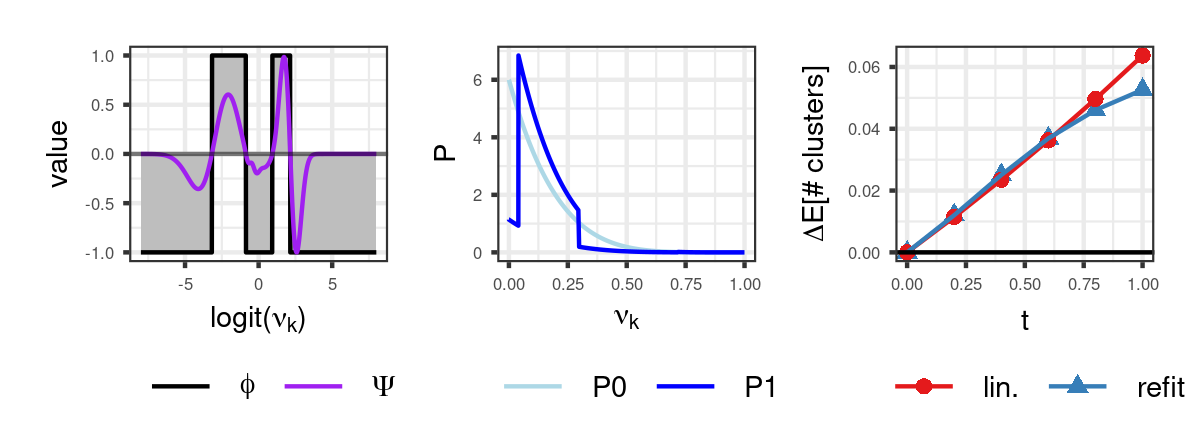
\includegraphics[width=0.784\linewidth,height=0.345\linewidth]{figure/iris_worstcase-1} 

}



\end{knitrout}
}


%%%%%%%%%%%%%%%%%%%%%%%%%%%%%%%%%%%%%%
%%%%%%%%%%%%%%%%%%%%%%%%%%%%%%%%%%%%%%
% Do not edit the TeX file your work
% will be overwritten.  Edit the RnW
% file instead.
%%%%%%%%%%%%%%%%%%%%%%%%%%%%%%%%%%%%%%
%%%%%%%%%%%%%%%%%%%%%%%%%%%%%%%%%%%%%%



%%%%%%%%%%%%%%%%%%%%%%%%%%%%%
% initial fit for structure
%%%%%%%%%%%%%%%%%%%%%%%%%%%%%
\newcommand{\StructureFit}{

\begin{knitrout}
\definecolor{shadecolor}{rgb}{0.969, 0.969, 0.969}\color{fgcolor}

{\centering 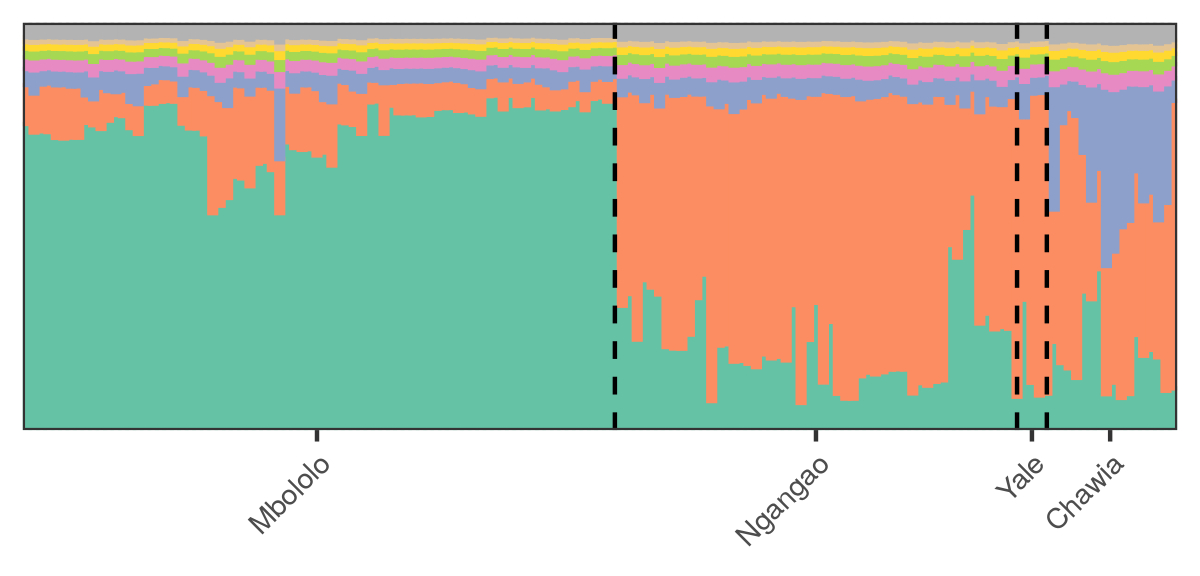
\includegraphics[width=0.980\linewidth,height=0.470\linewidth]{figure/structure_init-1} 

}



\end{knitrout}
}


%%%%%%%%%%%%%%%%%%%%%%%%%%%%%
% alpha sensitivity for structure
%%%%%%%%%%%%%%%%%%%%%%%%%%%%%
\newcommand{\StructureAlphaTreshZeroRefit}{

\begin{knitrout}
\definecolor{shadecolor}{rgb}{0.969, 0.969, 0.969}\color{fgcolor}

{\centering \includegraphics[width=0.980\linewidth,height=0.392\linewidth]{figure/structure_alphasens00-1} 

}



\end{knitrout}
}

\newcommand{\StructureAlphaTreshZero}{
\begin{knitrout}
\definecolor{shadecolor}{rgb}{0.969, 0.969, 0.969}\color{fgcolor}

{\centering 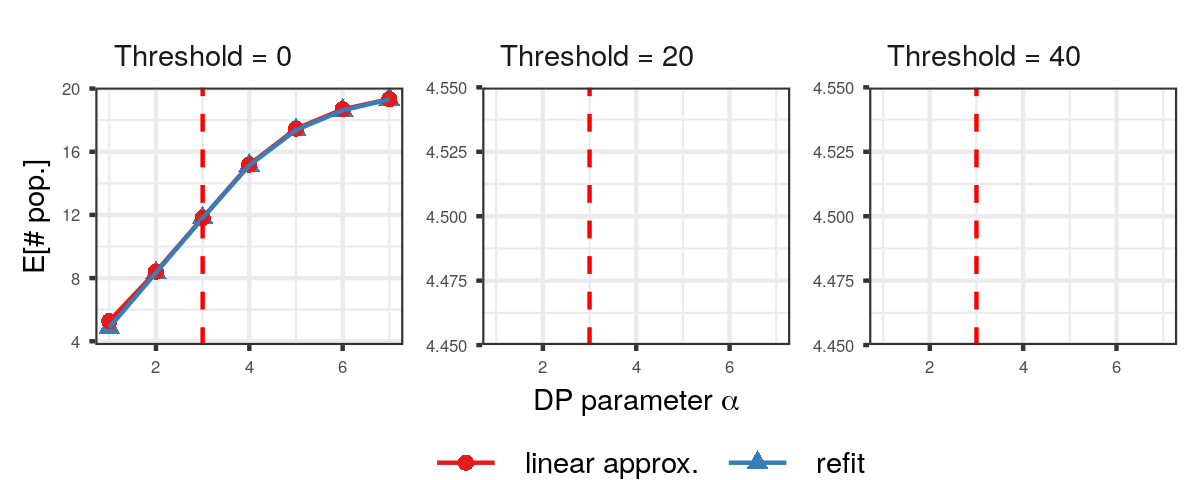
\includegraphics[width=0.980\linewidth,height=0.392\linewidth]{figure/structure_alphasens0-1} 

}



\end{knitrout}
}

\newcommand{\StructureAlpha}{
\begin{knitrout}
\definecolor{shadecolor}{rgb}{0.969, 0.969, 0.969}\color{fgcolor}

{\centering 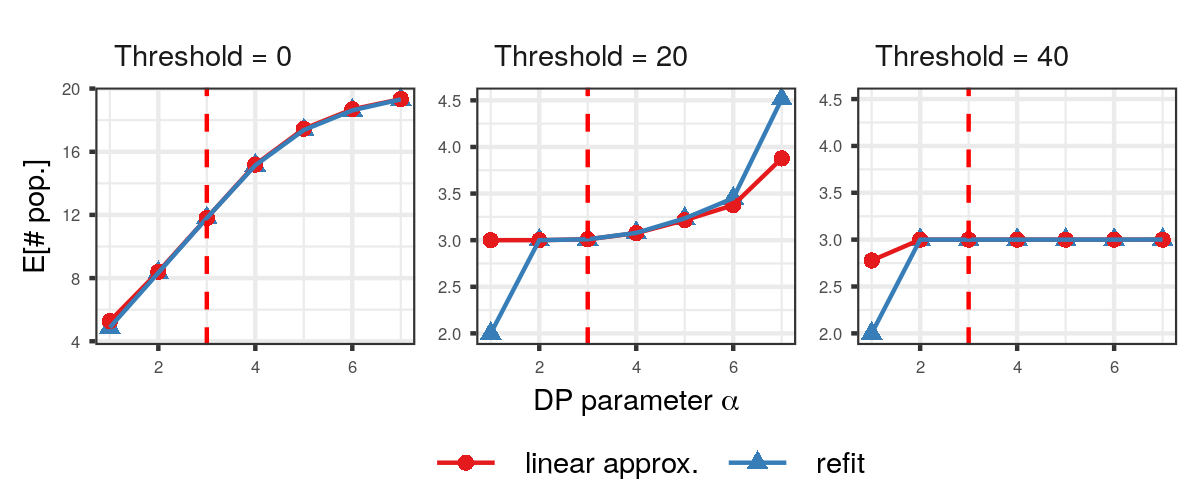
\includegraphics[width=0.980\linewidth,height=0.392\linewidth]{figure/structure_alphasens-1} 

}



\end{knitrout}
}

\newcommand{\StructureMigration}{

\begin{knitrout}
\definecolor{shadecolor}{rgb}{0.969, 0.969, 0.969}\color{fgcolor}\begin{kframe}


{\ttfamily\noindent\bfseries\color{errorcolor}{\#\# Error in eval(expr, envir, enclos): object 'mbololo\_box' not found}}\end{kframe}
\end{knitrout}
}


\newcommand{\MbololoOutliers}{

\begin{knitrout}
\definecolor{shadecolor}{rgb}{0.969, 0.969, 0.969}\color{fgcolor}\begin{kframe}


{\ttfamily\noindent\bfseries\color{errorcolor}{\#\# Error in eval(expr, envir, enclos): object 'mbololo\_box' not found}}

{\ttfamily\noindent\bfseries\color{errorcolor}{\#\# Error in eval(expr, envir, enclos): object 'p\_admix\_mbololo' not found}}\end{kframe}
\end{knitrout}
}


\newcommand{\NgangaoOutliers}{
\begin{knitrout}
\definecolor{shadecolor}{rgb}{0.969, 0.969, 0.969}\color{fgcolor}\begin{kframe}


{\ttfamily\noindent\bfseries\color{errorcolor}{\#\# Error in eval(expr, envir, enclos): object 'ngangao\_box' not found}}

{\ttfamily\noindent\bfseries\color{errorcolor}{\#\# Error in eval(expr, envir, enclos): object 'p\_admix\_ngangao' not found}}\end{kframe}
\end{knitrout}
}


\newcommand{\ChawiaOutliers}{
\begin{knitrout}
\definecolor{shadecolor}{rgb}{0.969, 0.969, 0.969}\color{fgcolor}\begin{kframe}


{\ttfamily\noindent\bfseries\color{errorcolor}{\#\# Error in eval(expr, envir, enclos): object 'chawia\_box' not found}}

{\ttfamily\noindent\bfseries\color{errorcolor}{\#\# Error in eval(expr, envir, enclos): object 'p\_admix\_chawia' not found}}\end{kframe}
\end{knitrout}
}

%%%%%%%%%%%%%%%%%%%%%
% limitations of local sensitivity 
%%%%%%%%%%%%%%%%%%%%%
\newcommand{\BadAdmixExample}{

\begin{knitrout}
\definecolor{shadecolor}{rgb}{0.969, 0.969, 0.969}\color{fgcolor}

{\centering 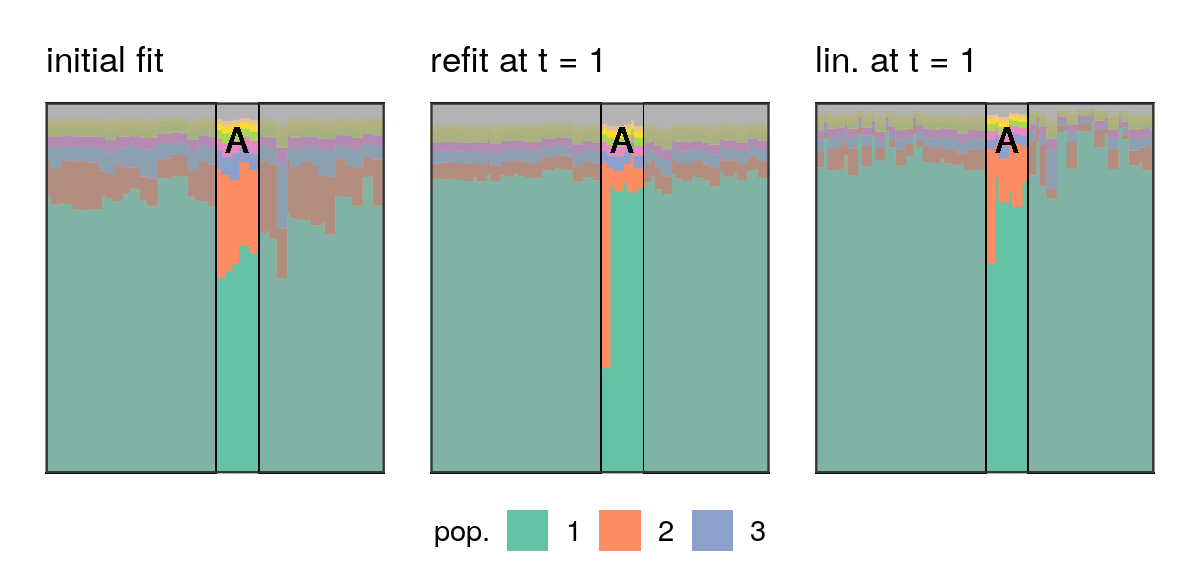
\includegraphics[width=0.980\linewidth,height=0.470\linewidth]{figure/bad_admix_ex-1} 

}



\end{knitrout}
}


\newcommand{\BadAdmixExampleTraceAdmix}{

\begin{knitrout}
\definecolor{shadecolor}{rgb}{0.969, 0.969, 0.969}\color{fgcolor}

{\centering 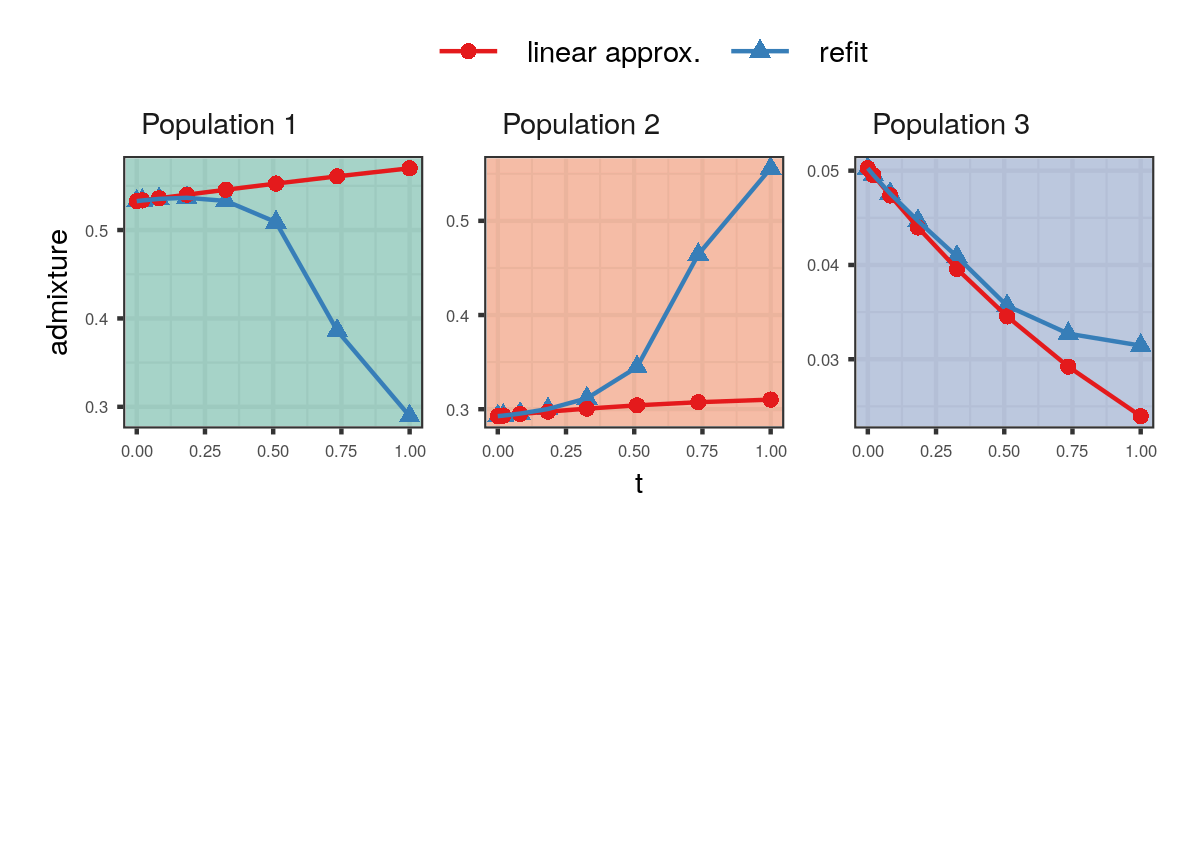
\includegraphics[width=0.980\linewidth,height=0.706\linewidth]{figure/bad_admix_trace_admix-1} 

}



\end{knitrout}
}

\newcommand{\BadAdmixExampleTraceAll}{
\begin{knitrout}
\definecolor{shadecolor}{rgb}{0.969, 0.969, 0.969}\color{fgcolor}

{\centering 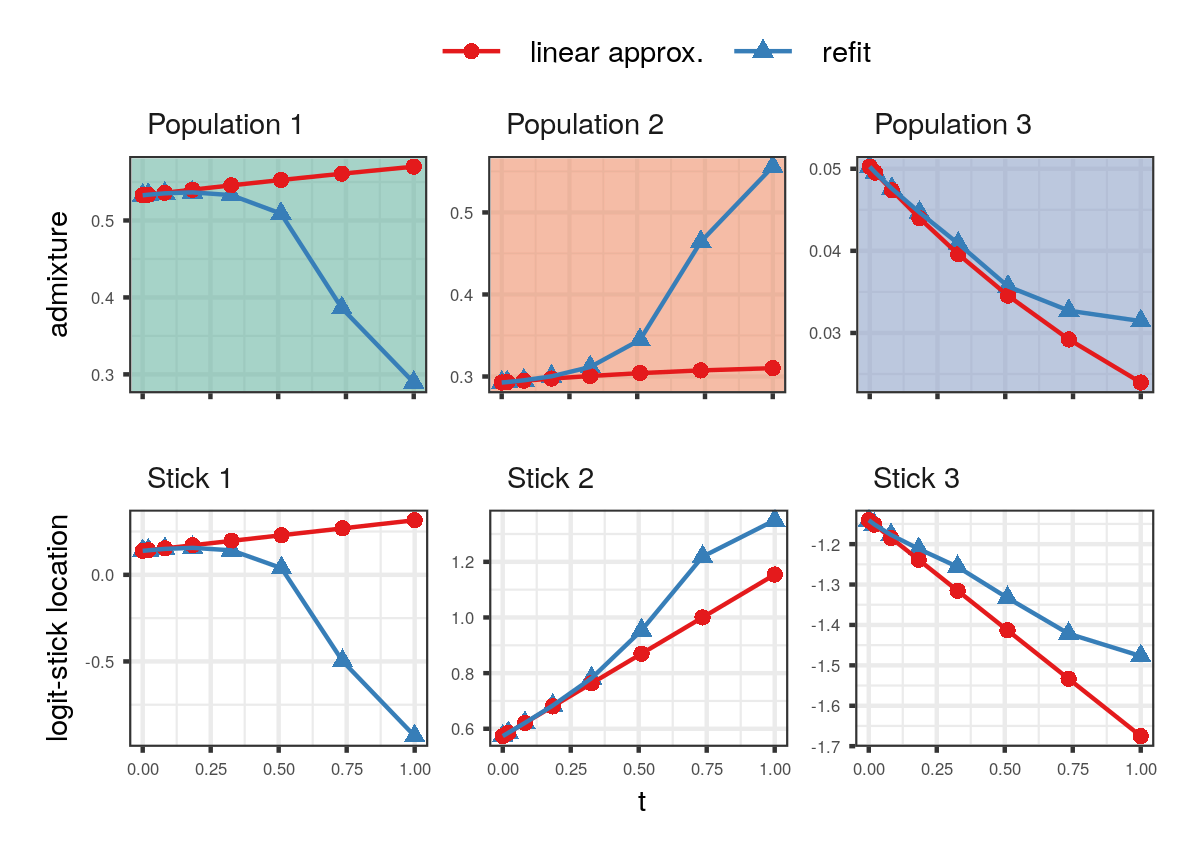
\includegraphics[width=0.980\linewidth,height=0.706\linewidth]{figure/bad_admix_trace_all-1} 

}



\end{knitrout}
}


%%%%%%%%%%%%%%%%%%%
% additional motivating example
%%%%%%%%%%%%%%%%%%%
\newcommand{\MbololoMotivatingExample}{

\begin{knitrout}
\definecolor{shadecolor}{rgb}{0.969, 0.969, 0.969}\color{fgcolor}

{\centering 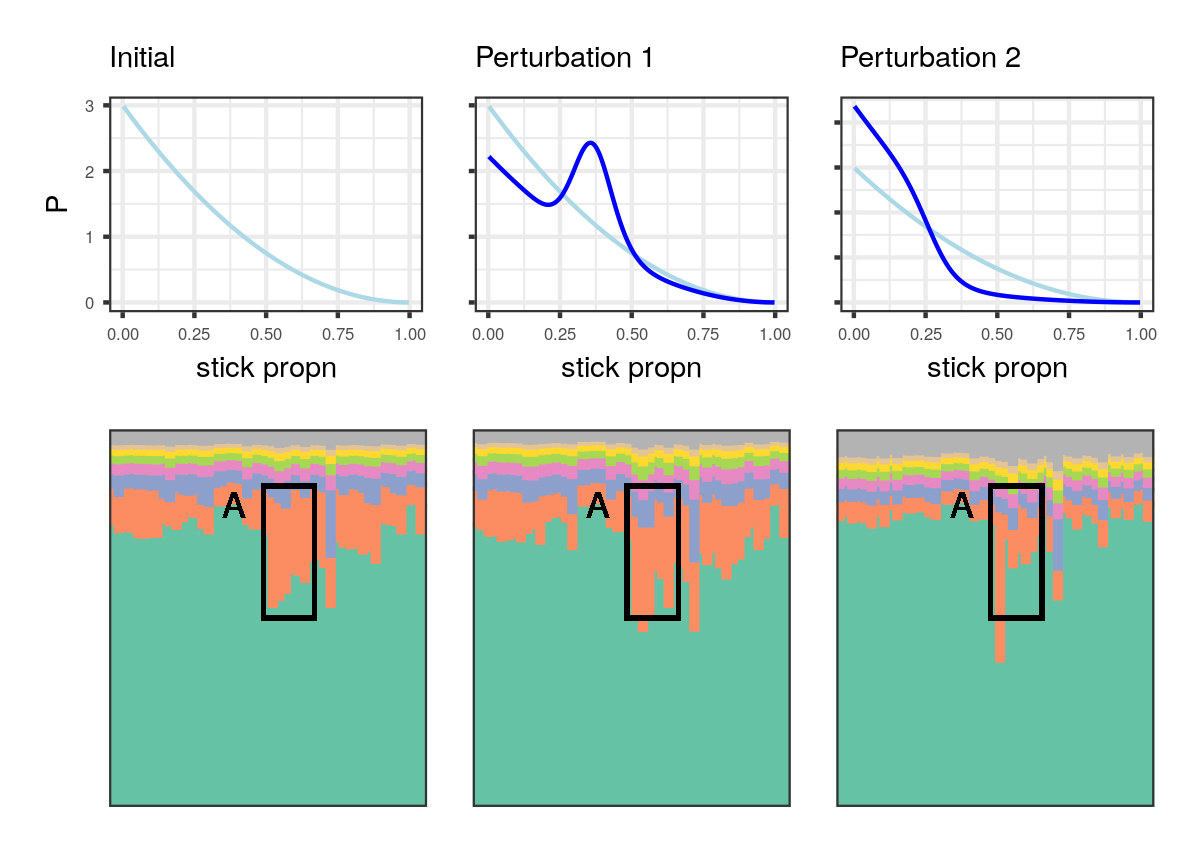
\includegraphics[width=0.980\linewidth,height=0.706\linewidth]{figure/mbololo_motivating_ex-1} 

}



\end{knitrout}
}

\newcommand{\MbololoMotivatingExampleInfluenceA}{

\begin{knitrout}
\definecolor{shadecolor}{rgb}{0.969, 0.969, 0.969}\color{fgcolor}

{\centering 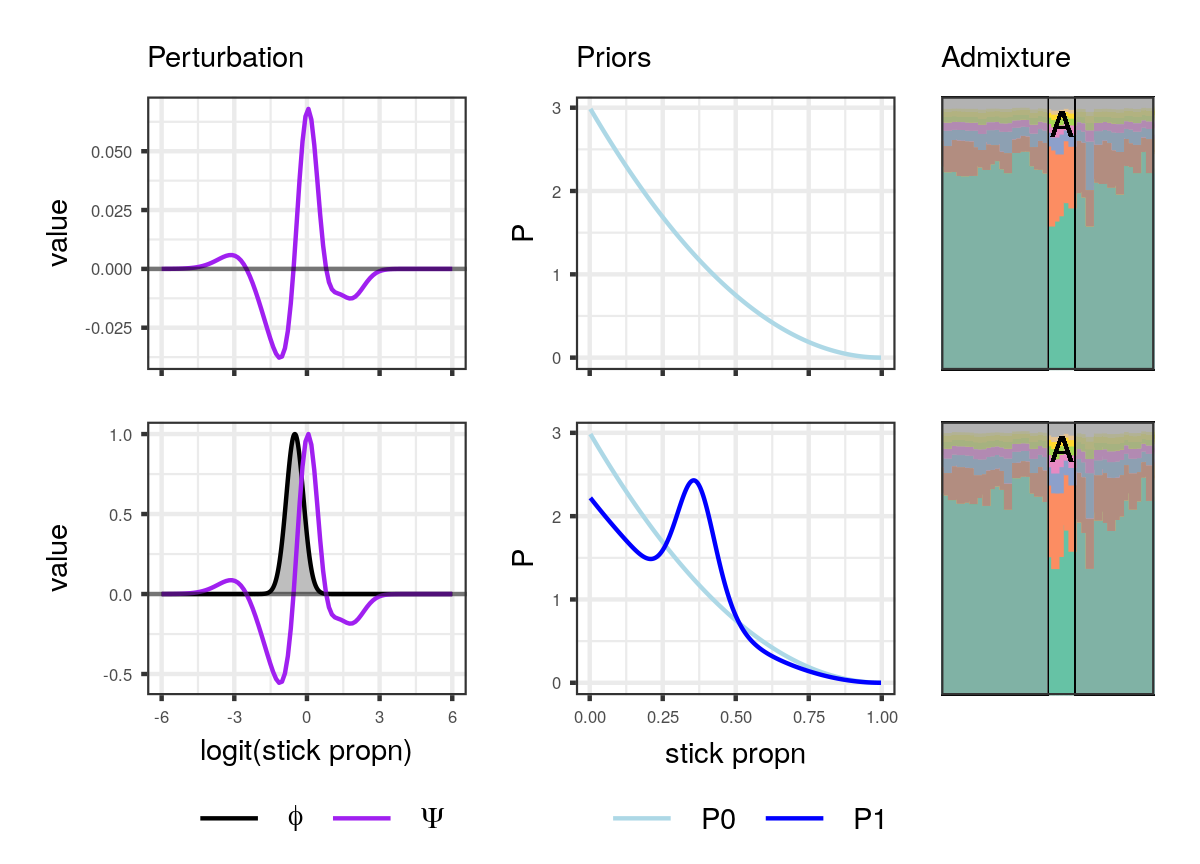
\includegraphics[width=0.980\linewidth,height=0.706\linewidth]{figure/mbololo_motivating_ex_inflA-1} 

}



\end{knitrout}
}


\newcommand{\MbololoMotivatingExampleInfluenceB}{
\begin{knitrout}
\definecolor{shadecolor}{rgb}{0.969, 0.969, 0.969}\color{fgcolor}

{\centering 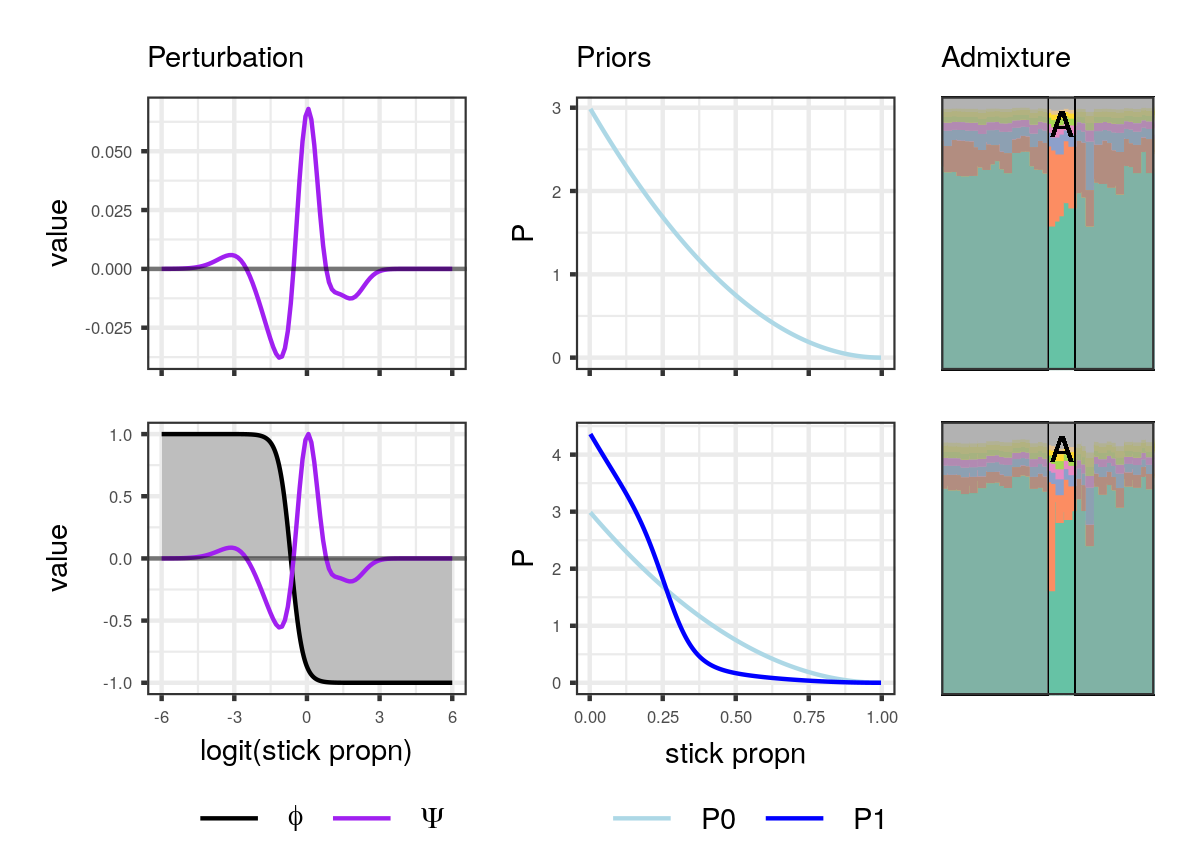
\includegraphics[width=0.980\linewidth,height=0.706\linewidth]{figure/mbololo_motivating_ex_inflB-1} 

}



\end{knitrout}
}







\begin{frame}
\FunctionPathsMultFig{}
\FunctionPathsLinFig{}
\end{frame}

\begin{frame}
\StructureFit{}
\end{frame}

\begin{frame}
\IrisFit{}
\end{frame}

\begin{frame}
\IrisAlphaRefit{}
\end{frame}

\begin{frame}
\IrisAlphaInSample{}
\end{frame}

\begin{frame}
\IrisAlphaAll{}
\end{frame}

\begin{frame}
\IrisInfluence{}
\end{frame}

\begin{frame}
\IrisFpertEx{}
\end{frame}

\begin{frame}
\IrisFpertAll{}
\end{frame}

\begin{frame}
\IrisWorstCase{}
\end{frame}

\begin{frame}
\StructureAlphaTreshZero{}
\end{frame}

\begin{frame}
\StructureAlpha{}
\end{frame}

\begin{frame}
  \StructureMigration{}
\end{frame}

\begin{frame}
  \MbololoOutliers{}
\end{frame}

\begin{frame}
  \NgangaoOutliers{}
\end{frame}

\begin{frame}
  \BadAdmixExample{}
\end{frame}

\begin{frame}
  \BadAdmixExampleTraceAdmix{}
\end{frame}

\begin{frame}
  \BadAdmixExampleTraceAll{}
\end{frame}

\begin{frame}
  \MbololoMotivatingExample{}
\end{frame}

\begin{frame}
  \MbololoMotivatingExampleInfluenceA{}
\end{frame}


\end{document}
